
The focus of this thesis is the characterization and calibration of superconducting qubits~\cite{Roth2021}.

The two words, \textit{characterization} and \textit{calibration}, are often used as synonyms, but it is useful to introduce a difference:
\begin{itemize}
    \item characterization means finding the values of \textit{intrinsic} properties of the qubit (for example its resonance frequency, its $T_1$...);
    \item calibration means finding the optimal parameters to \textit{control} the qubit.
\end{itemize}

The following parameters are the main ones to be obtained in characterization experiments:
\begin{description}
    \item[Qubit resonance frequency] The qubit resonance frequency refers to the specific frequency at which a qubit undergoes a transition between its first two energy levels. This parameter that determines the operational frequency of the qubit.
    \item[Resonator resonance frequency] The resonator resonance frequency is the natural frequency at which a resonator oscillates. This frequency is dependent on the physical characteristics of the resonator and is essential for readout operations.
    \item[Q factors] Quality factors measure the damping of oscillations in a resonant system. A high Q factor indicates minimal damping and high energy efficiency, while a low Q factor indicates significant damping. In the context of quantum systems, a high Q factor is desirable for maintaining coherence and prolonging the lifetime of quantum states. It is defined as $Q = \frac{f_r}{\Delta f_r}$
    \item[Coupling $g$ ] The coupling parameter $g$ represents the strength of the interaction between two quantum components, such as a qubit and a resonator. It determines the rate at which energy is exchanged between the components.
    \item[Dispersive shift] The dispersive shift is a phenomenon in quantum systems where changes in the energy levels of a qubit are observed due to its interaction with a resonator. This shift depends on the state of the resonator and can be used for qubit readout and manipulation.
    \item[Anharmonicity] Anharmonicity refers to the nonlinearity of the energy levels of a quantum system and signifies that the energy difference between different quantum states is not strictly equal.
    \item[Relaxation time $T_1$] The relaxation time $T_1$ characterizes the time it takes for a qubit to return to its ground state from an excited state. It quantifies the qubit's tendency to lose energy and coherence, often due to interactions with the environment.
    \item[Dephasing time $T_2$] The dephasing time $T_2$ represents the duration during which a qubit can maintain coherence without undergoing energy-changing transitions. It measures the qubit's resilience against fluctuations and noise in its environment.
\end{description}

As we can see, characterization parameters are intrinsic properties of the qubit system and come mostly from fabrication.\\
On the other hand, we have calibration experiments that analyze optimal control parameters:

\begin{description}
    \item[Drive frequency] The optimal frequency of the pulses required to change the state of the qubit.
    \item[Drive amplitude] The optimal amplitude of the pulses used to change the rotate the state of the qubit on the Bloch sphere, as well as the mapping between amplitudes and rotated degrees.
    \item[Drive duration \& shape] The optimal duration and shape of the control pulses to change the qubit state as required and minimizing leakage to higher excited states.
    \item[Assignment fidelity] Parameters to classify the states, zero and one, from IQ values as well with assignment fidelities.
    \item[Time of flight] time required for a signal to travel from the RFSoC to the qubit and back, required for pulse control and readout.
    \item[Readout frequency] The optimal frequency of the pulses required to read the state of the qubit.
    \item[Readout amplitude] The optimal amplitude of the pulses required to read the state of the qubit
    \item[Readout duration \& shape] The optimal duration and shape of the pulses required to optimize the read-out the state of the qubit
    \item[Gate fidelity] The accuracy relative to specific operation that differ from an exact matrix, by some measurable factor.
\end{description}

%In \cref{tab:calibration_parameters} some of the main parameters of calibration are listed.

%In \cref{tab:characterization_parameters,tab:calibration_parameters} are listed the main parameters to be obtained with characterization and calibration experiments.
%Although some concept may be unfamiliar, this should help distinguish the two processes, while more details will be given in the next sections.
%
%\begin{table}[ht]
%    \centering
%    \begin{tabular}{l|l}
%        Qubit resonance frequency &  Resonator resonance frequency\\
%        Q factors & Coupling $g$ \\
%        Dispersive shift & Anharmonicity \\
%        $T_1$ & $T_2$ \\
%    \end{tabular}
%    \caption{Main parameters to be obtained with characterization.}
%    \label{tab:characterization_parameters}
%\end{table}
%
%\begin{table}[ht]
%    \centering
%    \begin{tabular}{l|l}
%        Drive frequency &  Readout frequency\\
%        Drive amplitude & Readout amplitude \\
%        Drive duration \& shape & Readout duration \& shape \\
%        Assignment fidelity & Gate fidelity \\
%        Time of flight & \\
%    \end{tabular}
%    \caption{Main parameters to be obtained with calibration.}
%    \label{tab:calibration_parameters}
%\end{table}

The difference is often minimal and many experiments fall in both categories at the same time, but nevertheless the difference is substantial.
In particular, the objective of an experimenter may be just in characterization, so with no interest in optimizing the control of the qubit, or just in calibration, with only interest in reaching good control without interest in knowing parameters such as quality factors or coupling values.

In this chapter (and this thesis), I will try to give a description and some examples for all the most important experiments in single qubit characterization and calibration.
Note that the list hereby provided is not exhaustive at all and, in particular for calibration, the possible experiments are almost unlimited.

The main sources for this chapter, that are maybe more precise and advanced then this thesis are \cite{Gao2021, Kim2023, Naghiloo2019, Zijun2018}.\\
This chapter, on the other hand, tries to present the experiments in the clearest possible way, so that they can easily reproduced.
For every experiment, ideal and real-case plots are provided so that the reader can have a better grasp of the differences between the ideal situation and the reality.\\
Moreover, at the end of every experiment a short recap will be provided, in the form of a blue color box.

In the case of flux-tunable devices, some more experiments are needed: these experiments will always have names starting with "Flux ..." and will be differentiated by the others also by the use of a red recap box.
These experiment can/have to be avoided in the case of non-flux-tunable qubit characterization.

\begin{figure}[htbp]
    \centering
    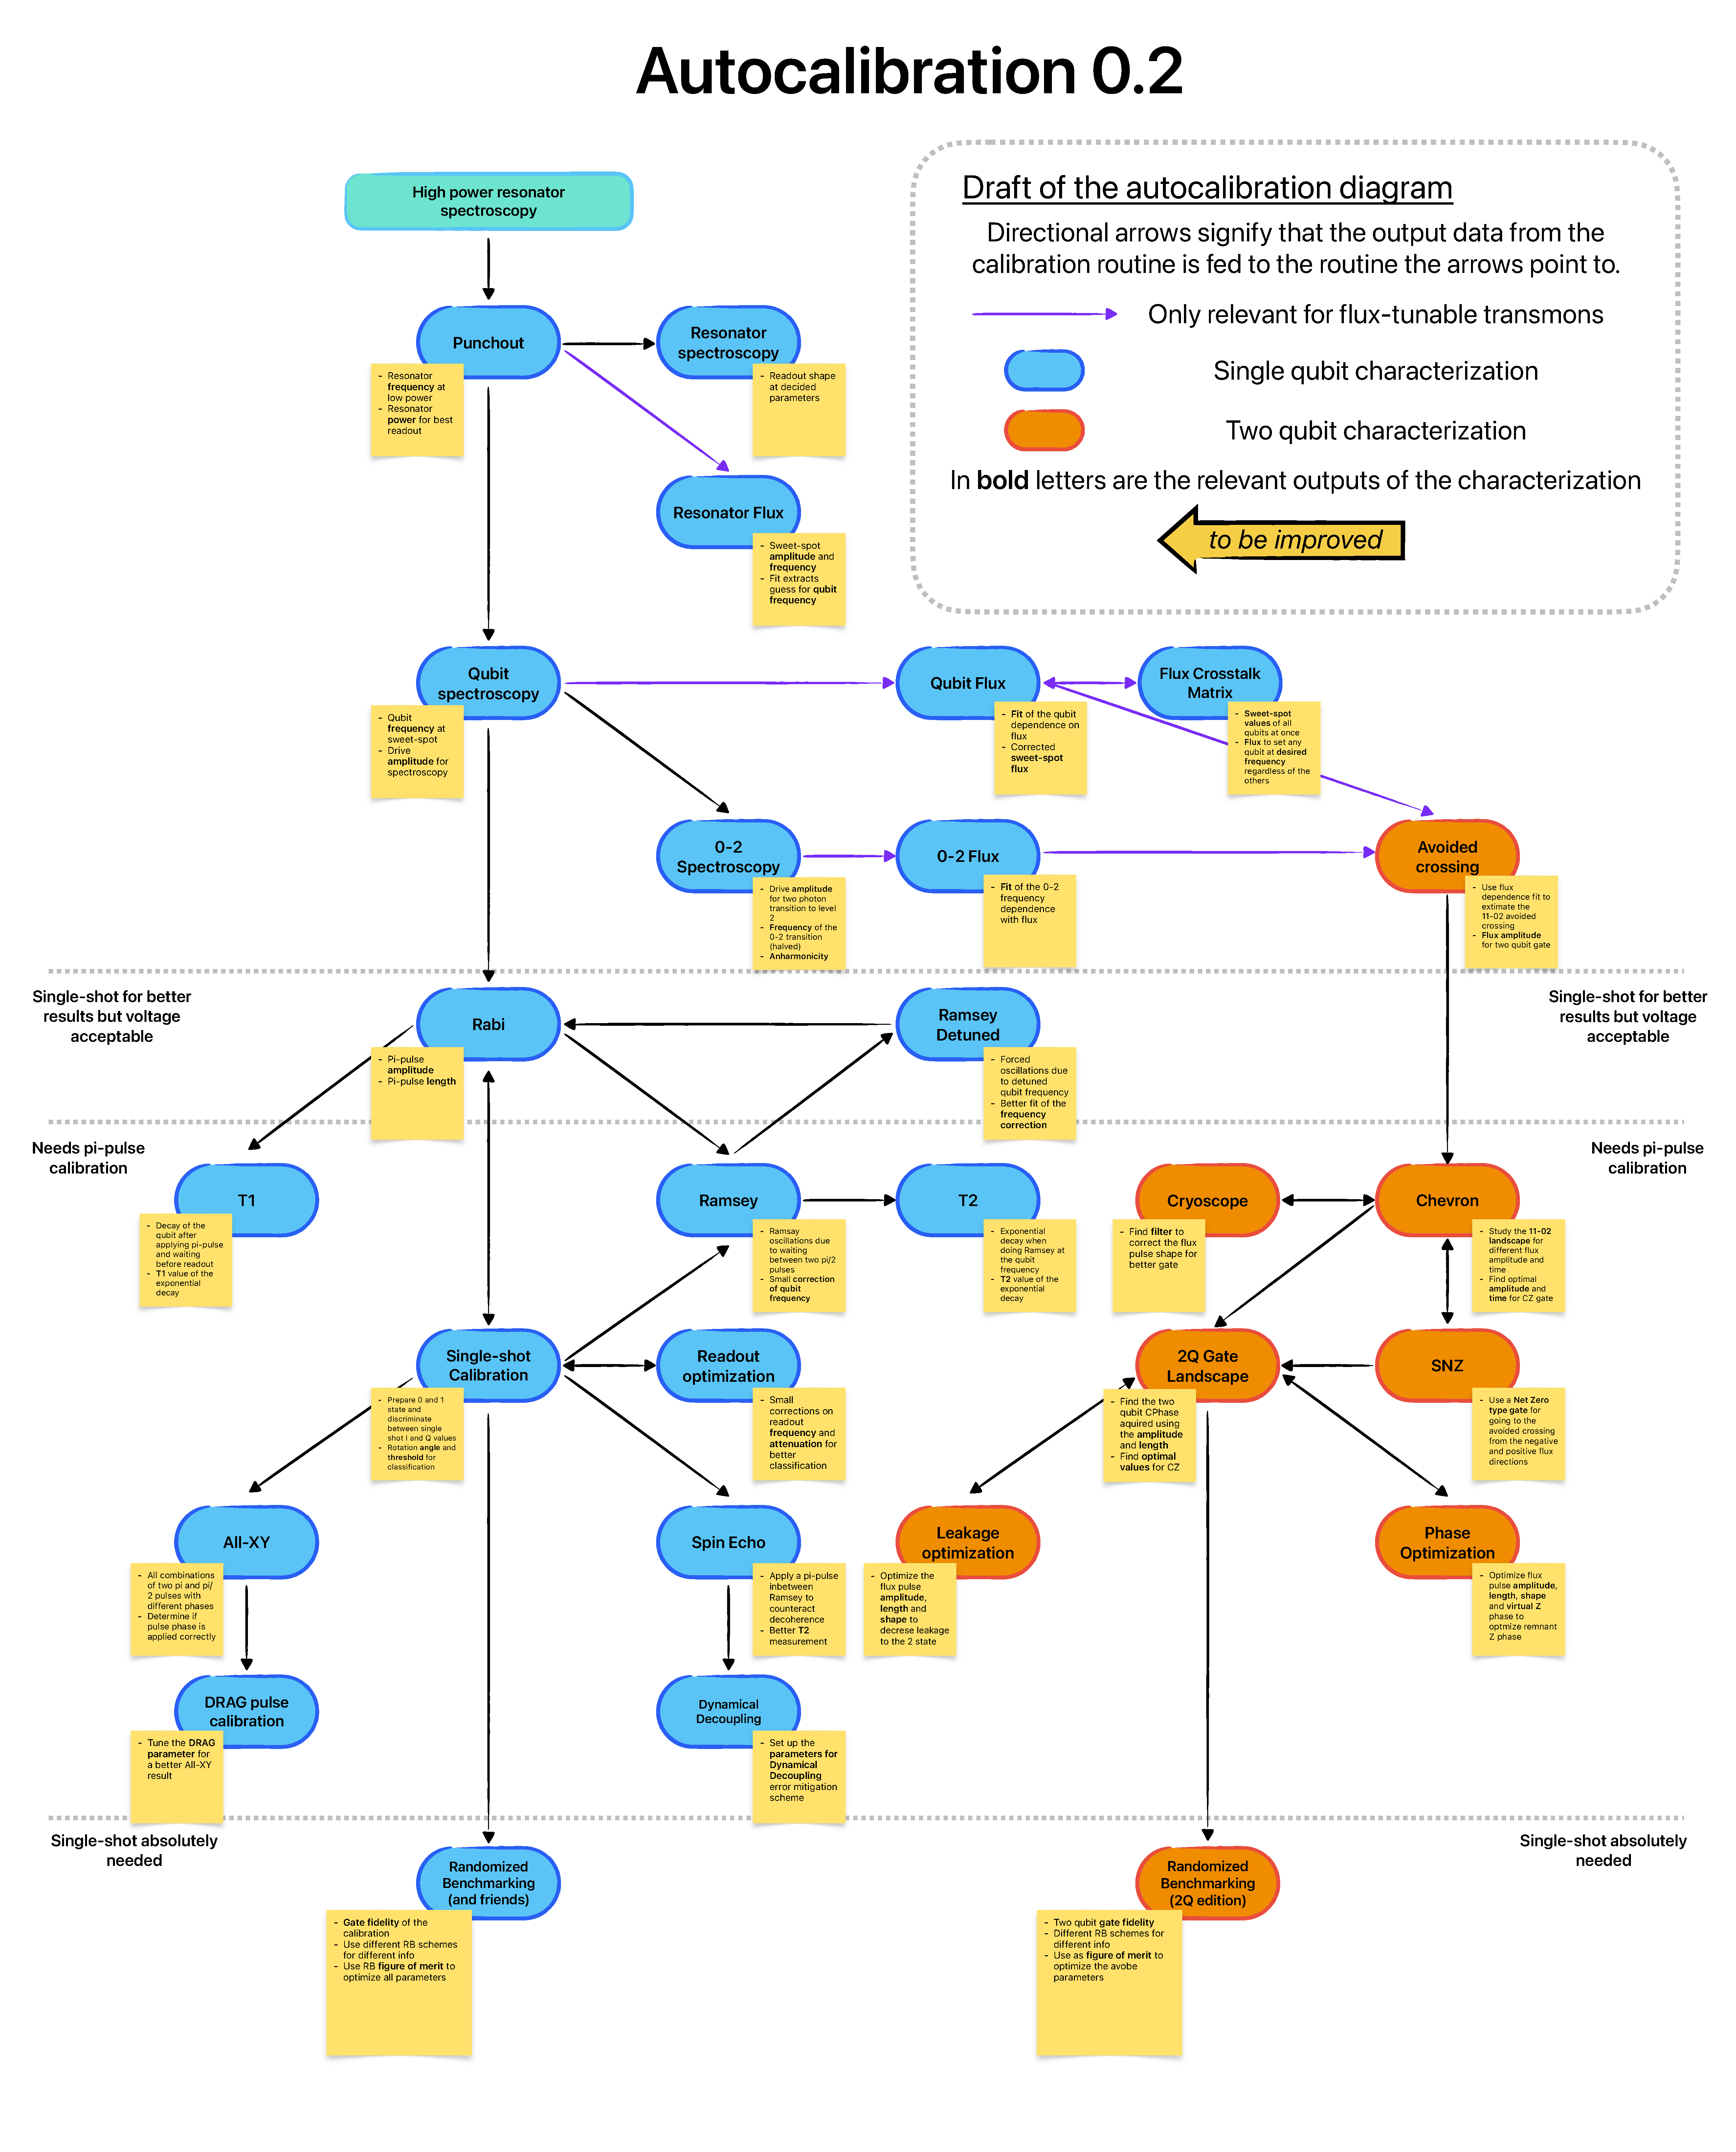
\includegraphics[width=\textwidth]{characterization/figures/Autocalibration 0.2.pdf}
    \caption{Scheme of the characterization and calibration experiments as presented for \Qibocal auto-calibration module.}
    \label{fig:scheme_experiments}
\end{figure}

In \cref{fig:scheme_experiments}, an outline of the main experiments described in this chapter is presented as per the proposal for the auto-calibration module of \Qibocal. Several experiments are mentioned in the scheme and not yet available, so not described in this thesis.

Note that, while they are in order of priority (top to bottom), characterization and calibration \textbf{is not} a sequential process.
It will happen many times, as an experimenter, to go back in the experiments tree and repeat some procedure, to better optimize some parameters.\\
The burden of understanding when to repeat an experiment is necessarily left to the reader/experimenter and the apparent sequentiality of this chapter is just a matter of simplicity.

\vspace{1cm}

\textbf{A note:} the majority of the plots presented in this chapter are produced by \Qibocal and shown here complete of a left amplitude plot and a right phase plot.
Our discussion will always focus only on the amplitude plot for simplicity, but it has to be clear that the majority of information can also be extracted from the phase plot.
In the end, there is direct amplitude measured, but always two I-Q values from which we can compute amplitudes and phases.